\section{Components of XAI word extraction}
Components are
\begin{itemize}
	\item XAI method used
	\item Tokenizer
	\item (Pretrained) AI model used
	\item NLP task
\end{itemize}

It is readily seen that these components are not independent of each other.
Some completely determine the choice of another, while others limit the selection of the other components.
	[describe dependencies between components]
Task $\rightarrow$ model $\rightarrow$ tokenizer $\rightarrow$ words.

must investigate comparability of results later.

(also corpus $\rightarrow$ task)
\subsection{Preliminary investigations of integrity}
The core idea this paper is to evaluate word utility by investigating a function (in the form of an AI model) that presumably represents some level of understanding of the language and checking which inputs (words) have the biggest influence on either the input or the model's internal state.
To ensure the function does possess this understanding, it is necessary to first ensure that the output of the model corresponds reliably to the ground truth, in other words, to tests the performance of the model on the specific data that will later be used to investigate the model itself.

\todo{A lot of prelim. test results, for example, first tests of NSP model on opensubs sentences show low reliability. Might also have to move this section to end (or in "results" chapter?)}


\subsection{Formal problem statement for XAI word extraction}

Givens:

\begin{itemize}
	\item A set $W$ of $w$ candidate words: $|W| = w$.

	\item A corpus $C$ containing lines/sentences in the target language.

	\item A function $f$ indicating the performance at the chosen task when given the subset of $W$
	      \begin{align*}f : 2^{W} \to \mathbb{R} \\
		      f (K) \mapsto p
	      \end{align*}

	\item An integer $k$ denoting the desired cardinality of the (smaller) subset of words to learn.
\end{itemize}
Find
\[
	\argmax_{K} f(K)
\]
\begin{align*}
	K \subset W \\
	|K| = k     \\
	k < |W|
\end{align*}

In practice, it is often not feasible to calculate calculate $f$ for every possible subset $K$, necessitating the use of approximations.



\section{NLP tasks}
The choice of NLP tasks employed to test a XAI-based approach for word utility estimation is a crucial step:
Since we are trying to estimate the utility a word a word has to language understanding, the NLP tasks should reflect language understanding as much as possible.
A good place to start looking for such tasks are those which are typically employed for pre-training NLP models:
Pre-training tasks are used to first endow the AI model with a general understanding of the language, before using transfer learning to specialize it for a more specific downstream task.
Such tasks must necessarily be general and require general language understanding, since training the model with them is supposed to provide a solid basis for a wide variety of NLP tasks.
\todo{Look at various pre-training tasks, preferably those used by state-of-the-art AI models}

\subsection{NLP pre-training tasks used by state-of-the-art AI models}
This section takes a look at the pretraining process of recent state-of-the-art LLM models which have made public their training process.
Both the NLP tasks and the kind of data is considered.


\begin{description}
	\item[GPT-4] \cite{openaiGPT4TechnicalReport2024}

	      Task: Language modeling (see next section).

	      Data: Not disclosed in detail, according to the original paper, the model was trained "using both publicly available data (such as internet data) and data licensed from third-party providers".
	\item[GPT-3] \cite{brownLanguageModelsAre2020}
	      GPT-3 is a model that does not rely on transfer learning to apply its linguistic understanding to new tasks; instead, it uses zero-shot and few-shot learning to perform tasks it was not specifically trained for.

	      Task: Language modeling (same as GPT-2 \cite{radfordLanguageModelsAre2019})

	      Data: Common Crawl, WebText2, Books1, Books2, Wikipedia \todo{link sources?}
	\item[LLama 3.3] \cite{LlamamodelsModelsLlama3_3}


	      Task: Meta did not make public the training process for Llama 3.3.

	      Data: "data from publicly available sources"
\end{description}

\subsection{Tasks considered}
\begin{description}
	\item[Next Sentence Prediction]
	      In this task, the AI model takes as input two sentences and predicts a probability for the second sentence being the successor of the first sentence in their source text.
	      Advantages for this task for our purposes is that such a dataset is easy to generate, as it merely requires a corpus of sentences that follow from each other, which is easily obtained from Wikipedia articles, film subtitles, or any other continuous text.

	\item[Text summarization]
	      This task involves summarizing a given text, in other words, writing a shorter version of the input text while still conveying as much of the information from the original text as possible.
	      Summarizing texts seems to require a high level of "understanding" of the text and would thus seem to be good choice for testing whether ablating certain words from the text would have detrimental effect on the model performance.
	      Unfortunately, this task requires hand-labeled datasets and is thus not a good candidate if we aim to find approaches which can be implemented in many different languages, as there is a dearth in data in many of the less-studied languages of the world.

	\item[Masked language modeling (aka. "cloze task")]
	\item[Causal language modeling (aka. Next token prediction)]
	\item[Sentence order prediction]
	\item[Sentence embeddings]
	      Sentence embeddings take the approach of transforming words into meaningful vectors and extend it to whole sentences.
	      This "task" differs from the others in that we do not measure differences in performance when the input is perturbed; but rather a distance between the embedding vectors themselves.
	      This justification for such an approach is that sentences whose meaning is very different should end up further apart from each other in the vector space once embedded.
	      This brings several advantages:
	      This approach can be performed on any corpus containing distinct sentences.
	      These corpus does not have to be document-level, and sentences need not be consecutive.
			To make this a task on which XAI methods can be applied, we can define a distance from the original token
\end{description}

\subsection{Sentence embedding methods}

\begin{description}
	\item[LASER] \cite{artetxeMassivelyMultilingualSentence2019}
	\item[BERT] \cite{reimersMakingMonolingualSentence2020}
\end{description}

\subsection{Data required for each NLP task}
The various NLP tasks employed require certain types of corpora to be employed properly:

\begin{itemize}
	\item[Next sentence prediction]
	      Requires a corpus that contains consecutive sentences.
	      Furthermore, NSP typically predicts whether two sentences follow each other in a document, not a dialogue (see the data on BERT training \cite{kentonBertPretrainingDeep2019}).
	      This excludes movie subtitles from the possible corpora for this task.

\end{itemize}

\section{XAI methods}
\begin{itemize}
	\item Attention as Explanation
	      Advantages:
	      Model only needs to be run once per sentence.
	      Longer sentences do not lead to a much longer calculations
	      Disadvantages: Justification as explanation controversial.
	\item Single Token Ablation
\end{itemize}

\section{Tokenizers}
[explanation of why tokenizers are important, explain various possible definitions of "word"]
[explain why morphosyntactically rich languages necessitate word splitting to some extend]

In some XAI models, we are free to choose any tokenizer we like.
We can choose, for instance, to only use full words, or word parts in English.
In input perturbation XAI approaches, we can choose to mask any part of the input with the help of tokenizers.
For decomposition approaches, the model is not looked at as a black box but instead examined using model-specific methods such as attention or Layer-based Relevance Propagation.
In such approaches, only the calculations made by the model itself are available for analysis, which means we are not free to choose our own word-splitting approach independent from the model.
This is because these models are trained using a specific tokenizer in the preprocessing, and changing the preprocessing makes the model function incorrectly.


\section{AI models}
\begin{itemize}
	\item NSP-model ABC
	\item LLAMA?
\end{itemize}

\todo{tests of performance tests of models used with corpora used (e.g., if NSP prediction model is reliable)}

\section{Interdependencies between components used}

While the components described above can mostly be used in any combination, there are some important restrictions to keep in mind:

\begin{description}
	\item[Attention as XAI can only be used on transformers]
	\item[Tokenization (and thus selection of word candidates) is only independent on model used in input perturbation approaches]
		As a direct consequence of this, other XAI mechanisms like attention as explanation are only useful for our purposes if the AI model uses a tokenization approach that somewhat corresponds to human notions of words.
		If a model uses tokenization approaches where a token is a combination of any three letters, any list obtained that tries to order the tokens by utility, while meaningful, will not be useful for human vocabulary learning.
		Note that in such cases, we can postprocess the data obtained, by merging the tokens to human-readable words and taking the average or maximum attention score of the AI model's tokens.
	\item[]
\end{description}



\subsubsection{Metrics used}

\begin{description}
	\item [Sequential rank agreement (modified)] \cite{ekstromSequentialRankAgreement2015}: This metric is based on the deviations of some subset of the lists in the upper ranks.
	      It is important to note that this metric has an additional parameter "depth" which determines how many elements (from the top of the list) are considered.
	      It is therefore more helpful to view its results at various depths.
	      The original formula for this metric in the case of two lists is:
	      \[
		      a_{d} := a \text{ from start to rank } d
	      \]

	      \[
		      S_{d} := a_{d} \cup b_{d}
	      \]

	      \[
		      SRA_{d}(a, b) := \lambda \cdot \frac{\sum_{x \in S_{d}} \sigma ^2 \left( \left( r_{b}(x) \right) - \left( r_{a}(x) \right) \right)}{|S_{d}|}
	      \]

	      where \(\lambda\) is a normalization factor ensuring that \(\max(SRA) = 1\).
	      In its proposed form, this metric can only compare lists which contain the same set of unique elements, just in different orders.
	      In order to make it work on lists where this is not the case, one can set the "rank" of nonexisting elements to a value greater than the length of the lists, such as \(2 |a|\).
	      Another drawback of the metric is that the standard deviation of two numbers does not depend on their absolute value, only their difference.
	      However, to satisfy number 3 of the stated requirements, we can take the deviation of the logarithm of the ranks instead of the deviation of the ranks themselves, resulting in the formula

	      \[
		      r^{\prime}(x) :=
		      \begin{cases}
			      \mathrm{rank}_{b}(x) & \text{if } x \in b, \\
			      2 \cdot |a|          & \text{otherwise.}
		      \end{cases}
	      \]

	      \[
		      SRA^{mod}_{d}(a, b) := \lambda \cdot \frac{\sum_{x \in S_{d}} \sigma ^2 \left( \log (r^{\prime}_{b}(x))-\log(r^{\prime}_{a}(x))\right)}{|S_{d}|}
	      \]

	      For this modified version, \(\lambda\) can be calculated with:

	      \[
		      \lambda = \frac{1}{SRA_{d}(a, a^{*})},
	      \]

	      where \(a^{*}\) is a list such that \(a \cap a^{*} = \emptyset\).
	      % \item \textbf{Average overlap / rank-biased overlap} \cite{webberSimilarityMeasureIndefinite2010}: Compares ranked list and puts more emphasis on the top of the list than at the bottom. However, assumes that the elements of both lists are the same, i.e., that all elements of list A are also in list B and vice versa.
	      %
	      % \item \textbf{11-point interpolated average precision} \cite{manningIntroductionInformationRetrieval2008}: Uses set metric precision (though may also use recall or F1 score on various subsets of the list (first 10\%, first 20\% etc.) and takes their geometric mean to arrive at a single number.
	      %       As each of the elevent numbers is calculated on the partial subset of the list's elements starting at the first element, this means that changes in the top of the list affect more of these numbers and thus have a larger impact on the final calculated mean.
	      %       One drawback of this method is that precision measurement within the 10\% interval only takes into account set membership, not the order of words:
	      %       For a list containing 10,000 words, the evaluated intervals are words in the index intervals $\left[ 0, 1000 \right), \left[ 0, 2000 \right), ... ,\left[ 0, 10000 \right)$.  Differences of order within the first 1000 words are thus ignored.

	\item [Discounted Cumulative Gain]:
	      This formula outputs a value between 0 and 1, with 1 being given if both lists are identical, 0 when they have no elements in common, and values in between when there is partial overlap between elements and/or their order is different.
	      ${DCG_{p}} =\sum _{i=1}^{p}{\frac {rel_{i}}{\log _{2}(i+1)}}=rel_{1}+\sum _{i=2}^{p}{\frac {rel_{i}}{\log _{2}(i+1)}}$
\end{description}

\[
	rel_{i} :=
	\begin{cases}
		\frac{1}{rank_{b}(el_{i}) + 1} & \text{if } el_{i} \in b \\
		0                              & \text{otherwise}
	\end{cases}
\]
\subsubsection{Metrics rejected}
\begin{description}
	\item [Kendall rank correlation ] \cite{kendallNEWMEASURERANK1938b}: This metric is bounded between 0 and 1 and compares the ranks of the elements of two lists. However, it cannot handle elements that only occur in one of the two lists, and thus is not suitable for our purposes. It also does not distinguish between differences in the upper and lower parts of the lists.
	\item [Spearman's footrule] \cite{spearmanCorrelationCalculatedFaulty1910}: Rejected for the same reasons as Kendall rank correlation.
\end{description}


\subsubsection{Tests of applicability}
[Results of preliminary tests of various metrics on own lists such as rank switching ,replacement at bottom and top of list etc.]



\section{Corpora}
\subsection{Selection criteria}

For the purposes of this paper, it was desirable that the corpora used be:
\begin{itemize}
    \item representative of what language learners strive for
    \item available in many languages
    \item for background corpora: Document-level
    \item freely accessible
\end{itemize}

\subsection{Corpora used}
\begin{description}
	\item[OpenSubtitles Parallel Corpus]
	      This set of corpora contains parallel corpora:
	      Corpora which has text segments in one language aligned with the presumed translation of the segment in a second language.
	      Its sentences are generated from subtitles from the popular subtitle sharing platform \textit{OpenSubtitles} (https://www.opensubtitles.org/) and undergo various preprocessing and filtering steps as described in \cite{lisonOpensubtitles2016ExtractingLarge2016}.
	      These include:
	      \begin{enumerate}
		      \item Enforcing universal UTF-8 character encoding.
		      \item
		            Splitting and joining of sentences from their original subtitles blocks (the segments which appear on screen when watching the movie with its subtitle).
		            One such block may contain multiple sentences, or only a partial one.
		            There is thus a n-to-m-relationship between the blocks and sentences.
		      \item Checking and correcting possible spelling issues, especially ones arising from OCR (Optical character recognition) errors.
		      \item From available subtitles, identifying the subtitle pair which is most likely to be accurate in its alignments and free from errors such spelling, taking into account metadata such as user ratings of subtitles.

	      \end{enumerate}
		  One advantageous aspect of this corpus is that is contains many sentences that are sequential, which means we can generate a Next Sentence Prediction dataset from it (add hedging here since not all lines in corpus are sequential and even within the same movies there may will be pauses in the subs).
		  This corpus has been used to train machine translation models such as OPUS-MT \cite{tiedemannOPUSMTbuildingOpenTranslation2020}, a freely available set of transformer models for translation, including between low-resource languages. \todo{Not completely correct, the pipeline uses data from OPUS, not necessarily or specifically from OpenSubs}
		  While it is possible to reconstruct which movies the subtitle lines came from from information contained in the corpus, it is unfortunately not clear how these movies were selected in the first place.

	\item[Leipzig Wortschatz Corpora]
		Available in x languages

		But: data quality issues, methodology might be outdated

		\cite{goldhahnBuildingLargeMonolingual2012}
	\item[CCMatrix / NLLB]

\end{description}

The full process, as illustrated by the authors, can be seen in figure \ref{fig:opensubs pipeline}
As of 2025, the latest version of the corpus (v2018) contains aligned subtitles of 62 languages between each other.

\begin{figure}[H]
	\centering
    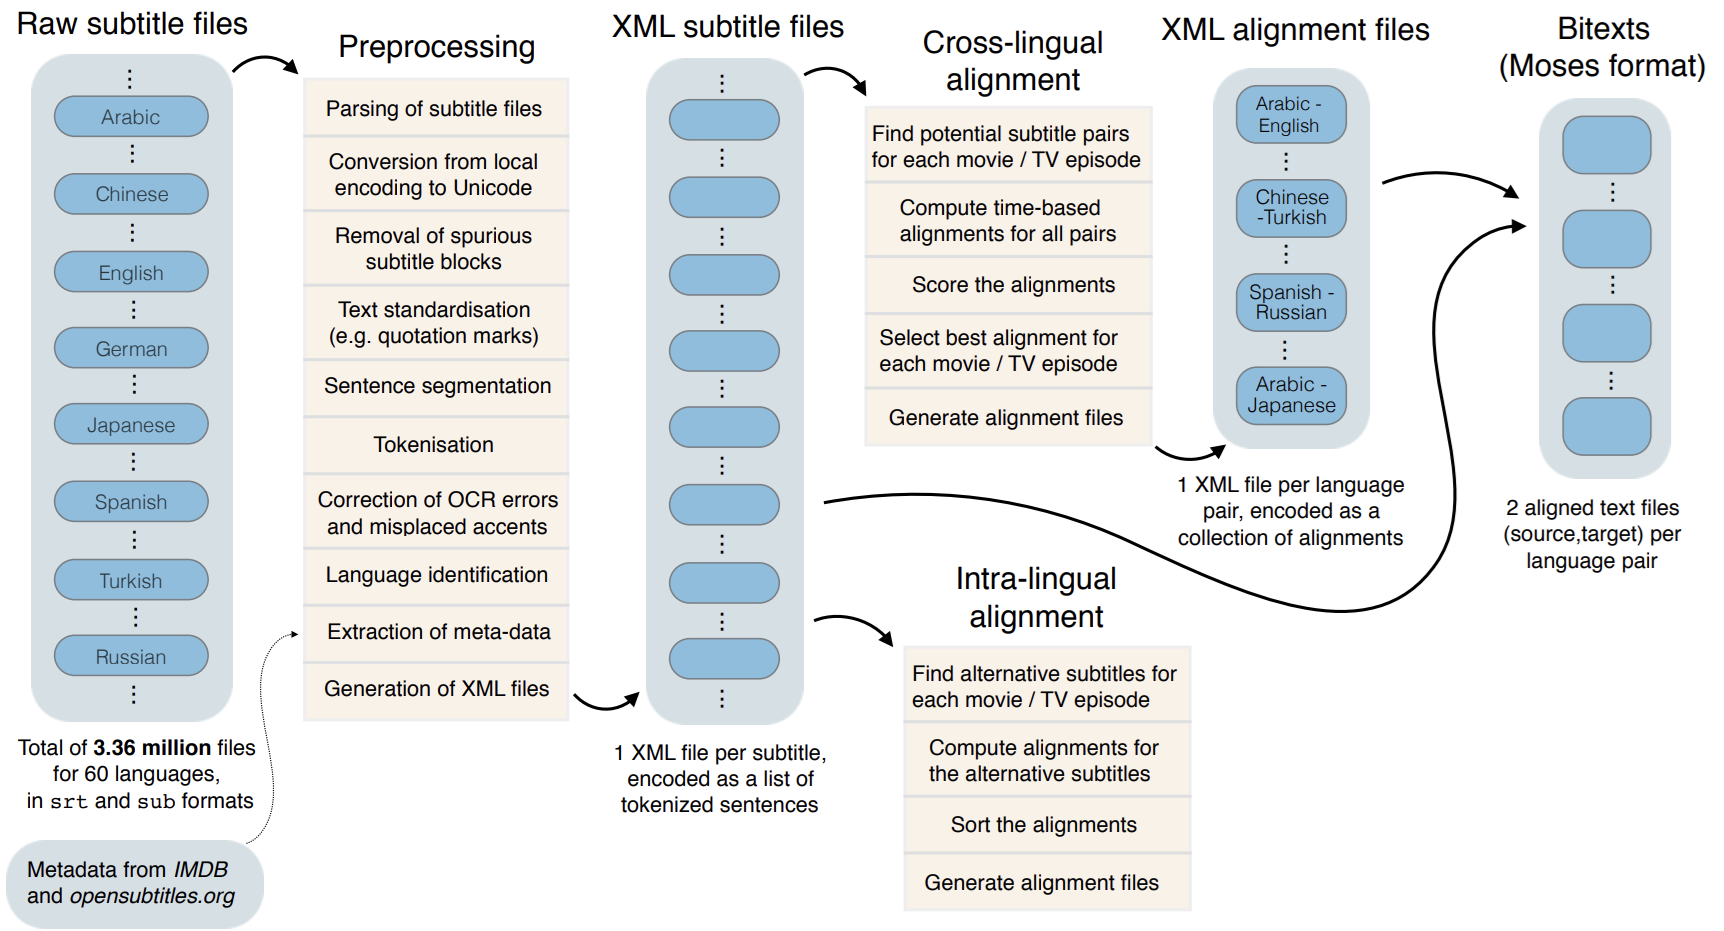
\includegraphics[width=\textwidth]{opensubs_corpus_processing.png}
	\caption{The pipeline producing the OpenSubtitles parallel corpus}
    \label{fig:opensubs pipeline}
\end{figure}

\section{Sources for existing lists for comparison}
It may be useful to compare the lists generated by the various approaches with existing word lists from educational materials:
Textbooks often feature chapters with word lists, or sentences which can be converted to word lists with a tokenizer.
The purpose is to have a point of comparison, to see if generated lists agree with existing lists, and find reasons for differences.

\begin{itemize}
	\item Language learning textbooks

	\item Language learning applications
	      \begin{itemize}
		      \item Duolingo: While Duolingo is the most popular language learning application as of 2024, it does not publish its word lists or course contents that is free of cost and easily convertible to a format that can be processed with NLP tools.
		      \item Rosetta Stone: Rosetta Stone publishes Course contents on its website. While the contents take the form of sentences, these can be converted to word lists by using a tokenizer on the contents and creating a list in the order in which they appear in the texts.
	      \end{itemize}
\end{itemize}


\section{Data Augmentation}
Data Augmentation was not used to gain additional data.
While in recent years data augmentation methods have become popular for training AI models in NLP, most of these would have either no or a detrimental effect on the methods employed in this paper:
Some of these methods include \cite{pellicerDataAugmentationTechniques2023}:
\begin{description}
	\item[Character level]
	      Introducing character swaps to data is a method used to train the model to noise in the data, but in our case, would only add noise to the results.
	\item[Word level]
	      There exist techniques to switch words for synonyms or swap words in the sentences to create noise.
	      As with noise on the word level, adding words in inappropriate places is undesired for our use case.
	      Swapping words for synonyms would also prove detrimental, as this would skew the statistics away from the natural word distribution found in the human-generated source texts.
\end{description}
Higher level techniques suffer from the same issues.
For this reason, the data is left in its "natural state" for our purposes.

